\documentclass[a4paper, 12pt]{article}
\usepackage{cmap}
\usepackage[utf8]{inputenc}
\usepackage[english, russian]{babel}
\usepackage[left=2cm, right=2cm, top=2cm, bottom=2cm]{geometry}
\usepackage{amsfonts,amssymb}
\usepackage{amsmath}
\usepackage{amsthm}
\usepackage{titlesec}
\usepackage{graphicx}
\usepackage{mathtools}
\usepackage{hyperref}

 \newcommand{\tit}[1]{\begin{center}{\bf{\Large #1}}\end{center}}
 \newcommand{\aut}[1]{\centerline{{\bf #1}}}
 \newcommand{\cityorg}[1]{\centerline{\it #1}}
 \newcommand{\email}[1]{\centerline{{\small e-mail: #1}}\vspace{\baselineskip}}
\providecommand{\keywords}[1]{\textbf{\textit{Ключевые слова:}} #1}
\newcommand{\norm}[1]{\left\lVert#1\right\rVert}
\newcommand{\normb}[1]{\left\lVert\textbf{#1}\right\rVert}

\begin{document}

\sloppy
 \tit{Макроскопическая маскирующая оболочка для видимого света}
 \aut{Baile Zhang, Yuan Luo, Xiaogang Liu, and George Barbastathis}

\begin{abstract}
Маскирующая оболочка являясь предметом, который обычно возникает в научной фантастике и мифах, недавно привлекла значительный интерес, в силу
своей возможной реализуемости. Самое большое известное испытания для
истинной невидимости ~--- маскировка макроскопического объекта в широком 
диапазоне длин волн, видимых для человеческого глаза. В этой работе
мы экспериментально решаем эту задачу для путем включения принципа
трансформационной оптики в традиционное построение оптических линз
при помощи дешевых материалов и простой техники изготовления.
Создана прозрачная оболочка, состоящая из двух частей кальцита.
Эта оболочка способна скрывать макроскопический объект, имеющий высоту
максимум 2мм, больший чем 3500 длин волн свободного пространства,
находящийся внутри прозрачной жидкой среды. Ее рабочий диапазон,
охватывающий красный, зеленый и синий свет, также продемонстрирован.
\end{abstract}

Среди различных устройств, концептуализированных в появившемся поле
трансорфмационной оптики~\cite{huanyang_review}, 
самым привлекательным может быть маскировочная
оболочка, которая может представлять объект невидимым путем точного
направления потока света вокруг объекта так, как будто бы объекта не
существует~\cite{leonhardt}-\cite{li_carpet}. 
Лежащий за этим механизм произрастает из формальной 
инвариантности уравнений Максвелла: преобразование координат не меняет вид 
уравнений, а изменяет только материальные параметры и значения поля.
Скрытый объект остается невидимым просто потому, что он находится вне
трансформированного электромагнетического пространства. Большой интерес
при реализации невидимости на практике вызвал массовые усилия в научных
исследованиях по микроволновым до оптических частот 
~\cite{schurig}-\cite{ergin}. 

Значительный прогресс был сделан в процессе исследования маскирующей оболочки.
Первая теоретическая модель оболочки, основанной на преобразовании координат 
~\cite{pendry}, требовала экстремальных значений использованных материальных 
параметров и могла работать только в очень узком диапазоне частот~\cite{pendry,
baile_rainbow}. Shuring  \textit{et al.} преодолели первый недостаток 
используя упрощенные параметры на
микроволнах, основываясь на технологии метаматериалов~\cite{schurig}. 
Чтобы преодолеть
ограничение на широту диапазона и сдвинуть рабочие частоты к оптическому
спектру, было предложено, что объект, помещенный на плоскую земляную
поверхность может быть невидимым, будучи помещенным под полностью непроводящую
gradient-refractive-index "ковровую"\ оболочку
(fully dielectic gradient-refractive-index carpet cloak), 
сгенерированную квазиконформным отображением~\cite{li_carpet}.
Эта модель оболочки-ковра
ведет к множеству последующих экспериментов в микроволновых
~\cite{ruopeng,huifeng} и инфракрасных частотах
~\cite{valentine,gabrielli,park,ergin}. 
Однако, недавно было указано серьезное
ограничение на ковровую оболочку: стратегия квазиконформного отображения
в целом ведет к боковому смещению рассеянной волны, чье значение сравнимо с 
высотой скрытого объекта, что делает объект 
обнаруживаемым~\cite{baile_lateral_shift}. Более того,
все предыдущие эксперименты по невидимости в оптическом спектре, от
инфракрасных~\cite{valentine,gabrielli,park,ergin} до 
видимых~\cite{smolyaninov_SPP,smolyaninov_waveguide} частот, были 
продемонстрированы под микроскопом, скрывая объекты, которые имели размеры, 
варьирующиеся от порядка 1 длины 
волны~\cite{smolyaninov_SPP,valentine,gabrielli,park,ergin} до, 
приблизительно, 100 длин волн~\cite{smolyaninov_waveguide}.
Как  "увидеть"\ эффект невидимости простым глазом, то есть спрятать
макроскопический объект для видимого света, все еще остается 
ключевым испытанием. В дополнение, большинство предыдущих оптических оболочек
~\cite{smolyaninov_SPP,valentine,gabrielli,park,ergin} требовали сложной нано 
или микроконструкции, в которой оболочка,
скрываемый объект и окружающая среда, служащая фоном, все были изготовлены
в одной структуре. Следовательно, они не могли быть просто отделены от их
встроенной структуры и перенесены куда-либо еще для сокрытия других объектов.
Эти ограничения, такие как обнаружимость, неадекватная производительность при
сокрытии больших объектов и непереносимость должны быть разрешены перед тем,
как оптическая оболочка станет практической.

\begin{figure}
\begin{centering}
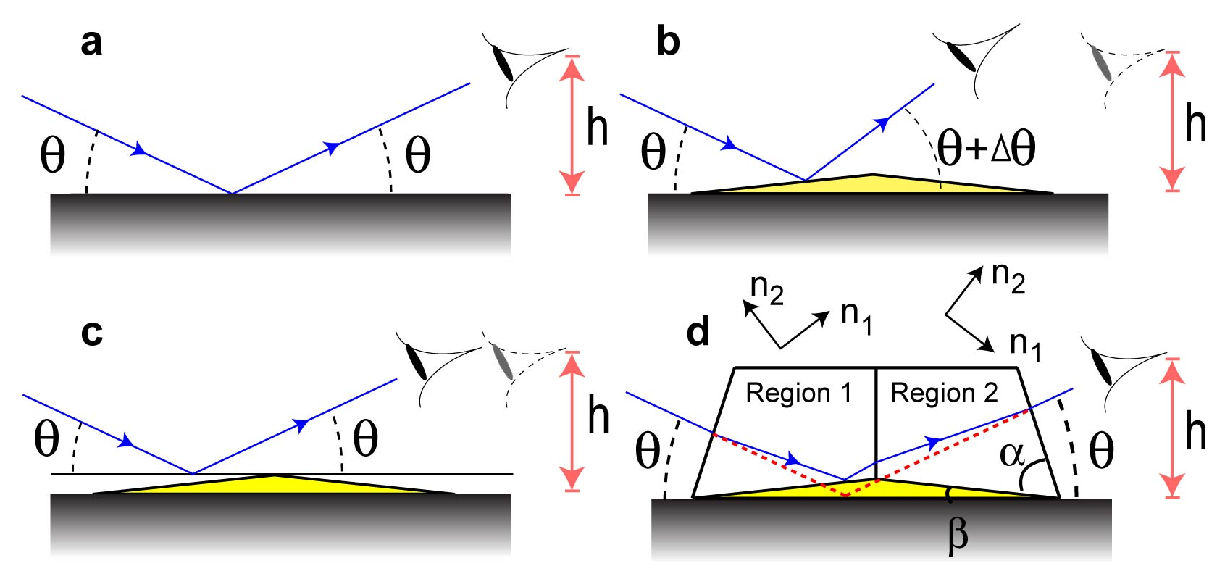
\includegraphics[width=0.7\columnwidth,draft=false]{Fig_1}
\caption{\label{fig:rays}  (a) Световой луч, падающий на плоскую земляную
поверхность и отраженный, под тем же углом.
(b) Когда объект расположен на поверхности, отраженный луч меняет угол. 
(c) Когда другая поверхность расположена сверху объекта, отраженный луч 
восстанавливает угол, но испытывает боковой сдвиг. (d) Когда основанная на 
преобразовании координат анизотропная оболочка покрывает объект, отраженный луч
восстанавливает и угол, и позицию. Анизотропная среда имеет два главных
показателя преломления $n_1$ и $n_2$ вдоль двух ортогональных направлений. 
Предполагается, что наблюдатель во всех случаях имеет фиксированную высоту $h$.
В (b) и (c) оригинальная позиция наблюдателя обозначена пунктирным глазом.}
\end{centering}
\end{figure}

\begin{figure}
\begin{centering}
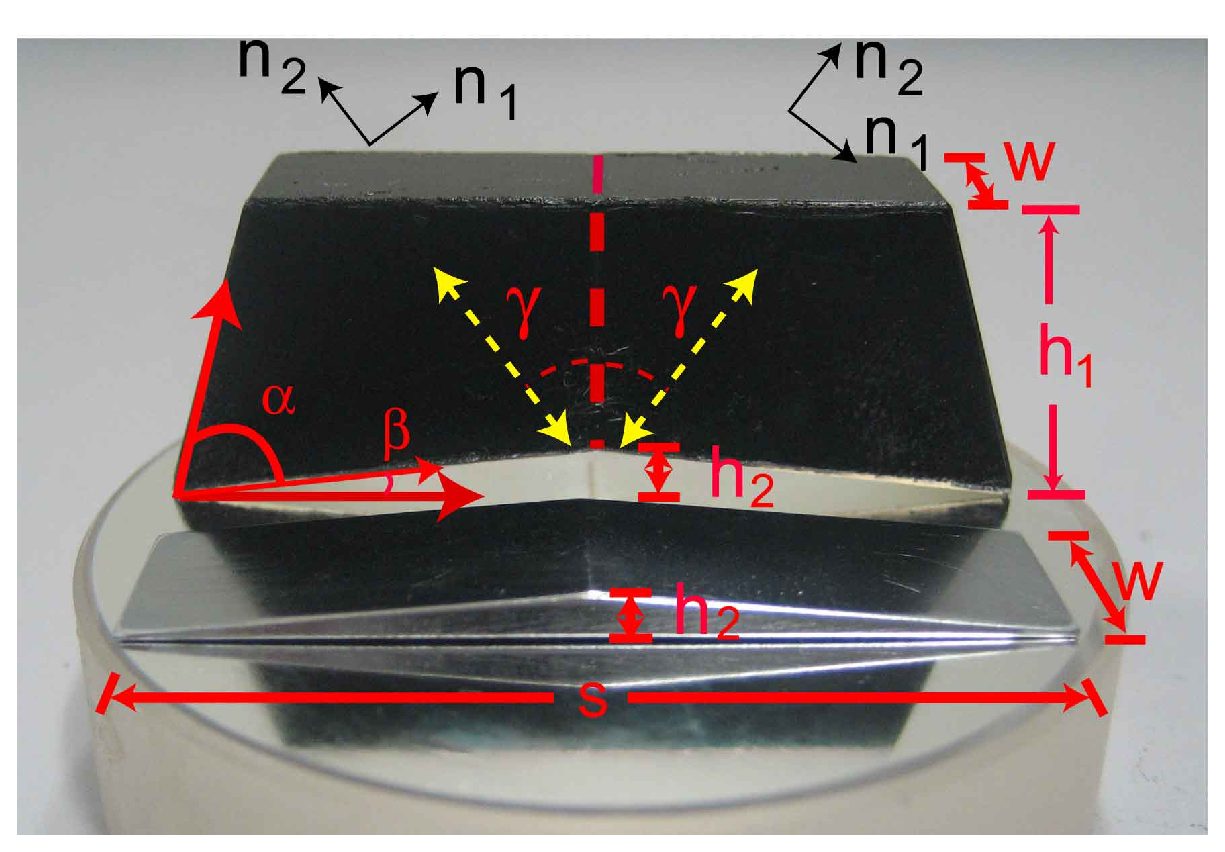
\includegraphics[width=0.7\columnwidth,draft=false]{Fig_2}
\caption{\label{fig:setup} Основанная на преобразовании координат
анизотропная оболочка, в сравнении с стальным клином, расположенным
на верхушке зеркала. Оболочка изготовлена из двух кусков кристалла кальцита
с специфической ориентацией оптических осей, обозначенной желтыми пунктирными
стрелками. Для зеленого света, с магнитным полем, перпендикулярным оптической 
оси, $n_1 = 1.48$ перпендикулярным оптической оси и $n_2 = 1.66$, направленным
вдоль оптической оси. $\alpha=66^{\circ}$, $\beta = 6^{\circ}$ и 
$\left|\gamma\right| = 37.5^{\circ}$. $w=10$ мм, $h_1 = 14.5$ мм, 
$h_2 = 2$ мм и $s=38$ мм.}
\end{centering}
\end{figure}

Вышеуказанные ограничения сводятся к двум трудностям при изготовлении
скрывающих материалов ~--- анизотропия и неоднородность. Предыдущая 
предложенная стратегия квазиконформного отображения пыталась решить
анизотропия для того чтобы изготовить метаматериальную 
реализацию~\cite{li_carpet}.
Однако, в традиционном построении оптических линз неоднородность
является более сложной для реализации, чем анизотропия. Пока еще остается
длинный путь, который стоит пройти, перед достижением практических 
применений нано-сконструированных метаматериалов, принцип трансформации
может быть напрямую встроен в традиционное изготовление оптических линз,
если преодолеть трудность неоднородности. Здесь, мы сообщаем о первой 
реализации макроскопической скрывающей оболочки для широкого диапазона
видимых длин волн путем применения дизайна трансформационной оптики для
в построении традиционных оптических линз. Оболочка сконструирована из
кальцита, обычного анизотропного оптического материала. Так как кальцит
сам по себе прозрачен в видимом свете, в этом случае не стоит заботится ни
о потери энергии для метаматериалов, так как она не существует, ни о 
ограничении на диапазон частот, связанный с ингридиентами 
метала~\cite{huanyang_review}.
Насколько нам известно, в нашем эксперименте невидимость была 
продемонстрирована впервые путем "видения"\ через оболочку напрямую,
то есть помещая целевой объект за оболочкой, подсвечивая систему видимым
светом, и показывая, что нет свидетельств присутствия замаскированного
объекта на изображении целевого объекта. И, следовательно, это ближайшая
к идеальной концепции оболочки реализация ~--- быть невидимой для глаза.

Чтобы объяснить дизайн нашей оболочки, сначала рассмотрим, почему объект
является видимым. Рис.~\ref{fig:rays}(a) показывает луч света, падающий
на земную поверхность под углом $\theta$. Как наблюдатель может видеть,
когда на поверхности ничего не находится, свет будет всего-лишь зеркально
отражен под тем же самым углом $\theta$ от поверхности. Когда на земную 
поверхность помещен объект, как треугольник на Рис.~\ref{fig:rays}(b),
отраженный свет изменит свой угол отражения. Это изменение может быть 
легко замечено наблюдателем. Самый удобный способом восстановления угла
отраженного света ~--- это поместить другую плоскую поверхность напрямую поверх
объекта, как показано на Рис.~\ref{fig:rays}(с). Однако, хотя угол и был 
восстановлен, отраженный свет испытывает заметный боковой сдвиг, который
раскрывает существование объекта. Поэтому, следовательно, важно восстановить
оба и угол, и позицию отраженного луча, чтобы отобразить объект невидимым
под оболочкой. Однородная оболочка треугольной формы, сделанная из одноосной
среды возможна, если электромагнитное пространство выше треугольного объекта
однородно сжимается сверху внутрь другого большого треугольника~\cite{xisheng},
так как оптический путь сохраняется при этом преобразовании. Для сохранения
материалов без существенного влияния на функцию маскировки, мы можем обрезать
оболочку до трапеции, с маленьким вытравленным снизу треугольником. Итоговая
структура показана на Рис.~\ref{fig:rays}(d). Важно, чтобы материалы
в регионах слева и справа имели бы два главных показателя преломления
$n_1$ и $n_2$, как отмечено на графике в~\cite{xisheng}. 
Фоновая среда должна иметь 
показатель преломления $n$, соответствующий значению между 
$n_1$ и $n_2$~\cite{zhang10},
хотя использование воздуха как фоновой среды тоже возможно~\cite{chen10}. 
Путь луча
на Рис.~\ref{fig:rays}(d) ясно показывает, что в диапазоне, ограниченном
урезанному размеру оболочки, произвольный падающий луч может быть идеально
проведен и выпущен под тем же углом, и с той же позицией, как на 
Рис.~\ref{fig:rays}(a). Это происходит потому, что анизотропная оболочка
эквивалентная сжатому электромагнитному пространству, в котором свет
"сбивают с толку"\, как если бы он распространялся в пустом пространстве
Рис.~\ref{fig:rays}(a), в котором ничего не лежит на земной поверхности.

Чтобы легко осуществить такую анизотропную маскировку на оптических частотах,
мы выбираем двумерную (2D) геометрию, в которой свет поляризован так, что 
магнитное поле параллельно горизонтальной опорной плоскости. Давайте сначала
рассмотрим следующее преобразование~\cite{xisheng} из оригинальных координат $(x, y)$
в новый набор координат $(x', y')$
\begin{eqnarray}
\begin{array}{c} x'=x;
\qquad
y' = \kappa y + \tau (a - |x|),
\end{array}.
\end{eqnarray}
где $\kappa = (\tan (\alpha + \beta)- \tan \beta) / \tan
(\alpha+\beta)$ и $\tau = \tan \beta$. 

Через это преобразование мы можем получить параметры для
материала в первом квадранте как
\begin{eqnarray}
\overline{\overline{\epsilon}}\:{}' & =  & \frac{\overline{\overline J} \cdot \overline{\overline{J}}^{T}}{|\overline{\overline J}|} = \left( \begin{array}{cc} 1/\kappa & -\tau /\kappa   \\
-\tau /\kappa & \kappa +\tau^2/\kappa
\end{array} \right); \\ 
\mu' & = & \frac{1}{\kappa},
\end{eqnarray}
где $\overline{\overline J}$ ~--- Якобиан преобразования. Материал во втором
квадранте имеет те же самые параметры, за исключением зеркального отражения 
по отношению к вертикальной плоскости.

\begin{figure}
\begin{centering}
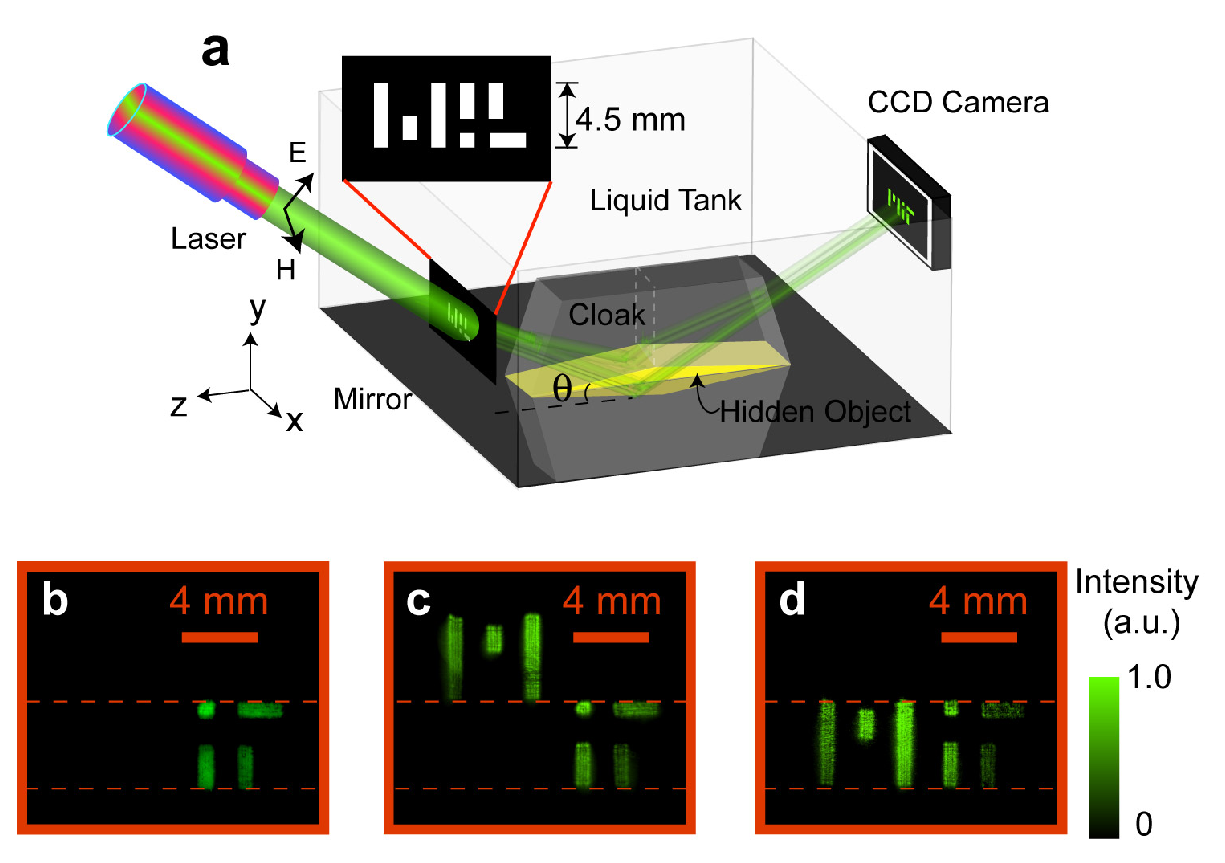
\includegraphics[width=0.7\columnwidth,draft=false]{Fig_3}
\caption{\label{fig:green} (a) Схематическая диаграмма экспериментальной
установки и изображений, полученных CCD камерой, (b) только с клином, но без
оболочки, (c) с плоской поверхностью, расположенной наверху клина, 
(d) с оболочкой наверху клина. }
\end{centering}
\end{figure}

Чтобы это работало с немагнитными материалами, мы масштабируем тензор
диэлектрической проницаемости таким образом, что
\begin{equation}
\overline{\overline{\epsilon}}\:{}'{}_{\text{nm}} = \left( \begin{array}{cc} 1/\kappa^2 & -\tau /\kappa^2\\
-\tau /\kappa^2 & 1 +\tau^2/\kappa^2\\
\end{array} \right).
\end{equation}
Это гарантирует, что $\mu'{}_{\text{nm}}=1$. Чтобы определить основные оси 
одноосного кристалла, мы диагонализируем 
$\overline{\overline{\epsilon}}\:{}'{}_{\text{nm}}$ и получаем ориентацию
осей кристалла по отношению к вертикальной плоскости в виде
\begin{equation}
\gamma = {1\over 2} \arctan \frac{2 \tau}{\kappa^2 + \tau^2 -1} \label{eq:gamma}.
\end{equation}

Чтобы зафиксировать геометрию, положим $\alpha = 66^{\circ}$ и 
$\beta = 6^{\circ}$, и получим $n_1^2=1.48^2$, $n_2^2=1.66^2$, и 
$\left|\gamma\right|=37.5^\circ$ для индекса преломления фоновой среды равного
1.57. Для зеленого света при длине волны 561 нм (где человеческий глаз наиболее
чувствителен в типичных средах~\cite{wyszecki}) и магнитном поле, ориентированным 
параллельно зеркалу, это можно легко реализовать как кальцит, с кристальной
осью, ориентированной согласно \ref{eq:gamma}.

Мы сконструировали экспериментальную оболочку, как показано на 
Рис.~\ref{fig:setup}. В силу ошибок изготовления в кристале кальцита, углы были
точны до $15'$, в то время как длина каждой стороны могла иметь ошибку до 1 мм.
Две части кальцита были вплотную зацементированы в месте, обозначенном 
пунктирной линией на Рис.~\ref{fig:setup}, при помощи 
Norland Optical Adhesive 61 ~--- чистого, бесцветного, жидкого фотополимера,
который лечит, находясь под воздействием ультрафиолетового света.
Передняя, задняя и верхняя поверхности оболочки были покрашены черным для
поглощения рассеянного света. Нижняя поверхность была полностью отполирована
и затем покрыта серебром. Левая и правая поверхности были полностью 
отполированы и служили как вход и выход для света, соответственно. В 
качестве скрываемого объекта был взят стальной клин, который подходил
пустоте под оболочкой, что так же показано на Рис.~\ref{fig:setup}.
В качестве альтернативы может быть взят любой меньший, чем этот стальной клин, 
объект. Так как дизайн нацелен на невидимость в прозрачной среде с показателем
преломления близким к $n=1.57$, значению, схожему с индексом преломления 
в~\cite{valentine},
это не является объектом ограничения задержек-пропускной способности и
задержек-потерь (delay-bandwidth, delay-loss) для маскировки в 
воздухе~\cite{hashemi}.

\begin{figure}
\begin{centering}
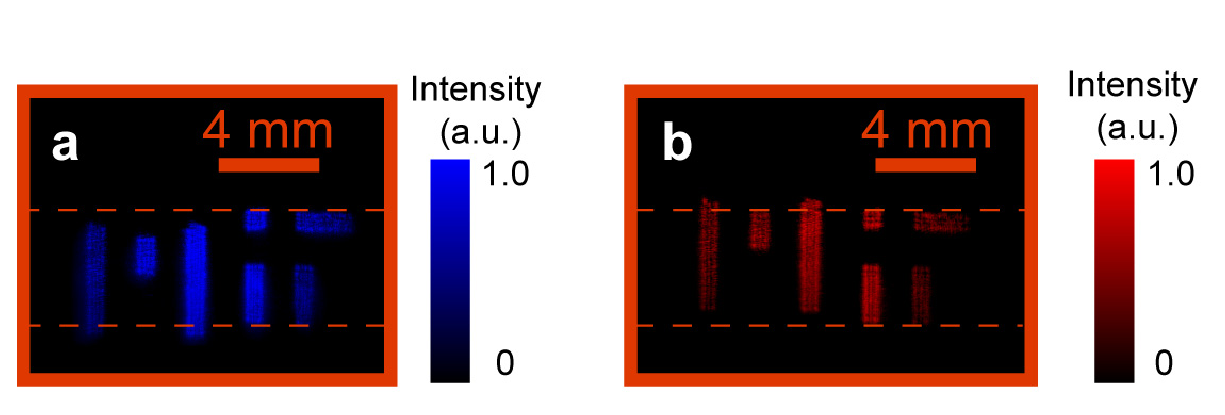
\includegraphics[width=0.7\columnwidth,draft=false]{Fig_4}
\caption{\label{fig:bluered} Изображения, полученные CCD камерой, когда 
оболочка покрывает клин и цвет свела измене на (a) синий, с длиной волны 488 
ни и (b) красный, с длиной волны 650 нм. Угол падения $\theta = 18^{\circ}$ 
внутри емкости.}
\end{centering}
\end{figure}

Как показано на Рис.~\ref{fig:green}, все объекты: оболочка, маскируемы клин
и зеркало, используемое как земная поверхность, были погружены в 
стеклянный контейнер, заполненный прозрачной бесцветной лазерной жидкостью
(OZ-Laser IQ, CODE 5610, от Cargille Labs, $n=1.53$,  измерено на длине волны
598.3 нм). Полый шаблон передачи с текстом "MIT"\ была напечатана на
непрозрачной пластиковой плате с толщиной 500 микрометров при помощи
стереолитографической машины (Viper$^{\rm TM}$ SLA System). В качестве
смолы был взят Accura 60 Plastic. Эта плата была инвертирована а затем
прикреплена клейкой лентой с левой стороны прозрачной емкости. В силу
конечной толщины платы, итоговое изображение "MIT"\ выглядит немного тоньше
в экспериментах.

Затем полый шаблон был подсвечен лазерным диодом с продолжительной волной (cw) 
на длине волны 561 нм, поляризованной так, что магнитное поле параллельно 
зеркалу. Позиция, на которой располагался шаблон была тщательно выбрана таким образом, что переданный через инвертированную "M"\ свет проходил через
оболочку с спрятанным под ней клином и отражался от низа оболочки, в то время
как свет, прошедший через "IT"\, отражался от зеркальной поверхности напрямую,
не задевая оболочку и клин. CCD (прибор с зарядовой связью) камера 
(Kodak ISS KAI-11002 с размером пикселя 9 микрометров) была помещена на 
расстоянии приблизительно 10 см от оболочки на правой стороне емкости.
Так как такая сделанная дома оболочка имеет сторонние ошибки до 1 мм,
в эксперименте мы подправили высоту оболочки, вставив стеклянную пластину, 
толщиной 100 микрометров под оболочку, чтобы минимизировать искажение 
изображений.

Маскировка в эксперименте на Рис.~\ref{fig:setup} и Рис.~\ref{fig:green}(а) 
доказывалась следующим образом: если оболочка может успешно скрыть клин, то
CCD камера должна зафиксировать прямую и недеформированную надпись "MIT"\,
как если бы на поверхности зеркала ничего не находилось. Мы выбрали угол
падения $\theta = 18^\circ$ внутри емкости по отношению к горизонтальной
опорной плоскости (внешний угол был исправлен в эксперименте, чтобы 
соответствовать номинальному значению $\theta$ согласно закону Снеллиуса).
Рис.~\ref{fig:green}(b) показывает изображение, полученное когда клин находится
на зеркале без оболочки. Буква "M"\, после отражения от клина находится очень
далеко от "IT"\ и не захватывается камерой. Рис.~\ref{fig:green}(с) показывает
изображение, полученное когда на вершине клина находится плоская поверхность.
Мы можем видеть что "M"\ сама по себе не искажена, но сдвинута вверх, по
сравнению с "IT"\, по той же причине как на Рис.~\ref{fig:rays}(c).
Рис.~\ref{fig:green}(d) показывает изображение, полученное когда на верх
клина помещена оболочка. Все буквы запечатленного изображения расположены
на той же высоте, как если бы скрытый клин здесь не присутствовал. Чтобы 
убедится, что позиция, на которой свет отражается от низа оболочки не влияет
на эффект маскировки, мы сдвинули позицию оболочки вдоль оси $z$. Не было
обнаружено никаких очевидных дополнительных искажений, кроме отражения,
возникшего вдоль линии сопряжения между двумя частями кристалла кальцита.

Плоская поверхность земли для Рис.~\ref{fig:green}(с) была изготовлена 
следующим образом: сначала, мы поместили плоскую стальную плату высотой 2 мм
близко к клину. Затем, мы поместили кусок стекла толщиной 1.5 мм с одной 
стороны покрытый хромом на поверхности, с покрытой стороной затрагивающей
оба: и пик клина, и плоскую поверхность. Так как индекс преломления стекла 
почти полностью совпадал с средой жидкости лазера, эта толщина имела 
незначительное влияние на экспериментальные результаты.

\begin{figure}
\begin{centering}
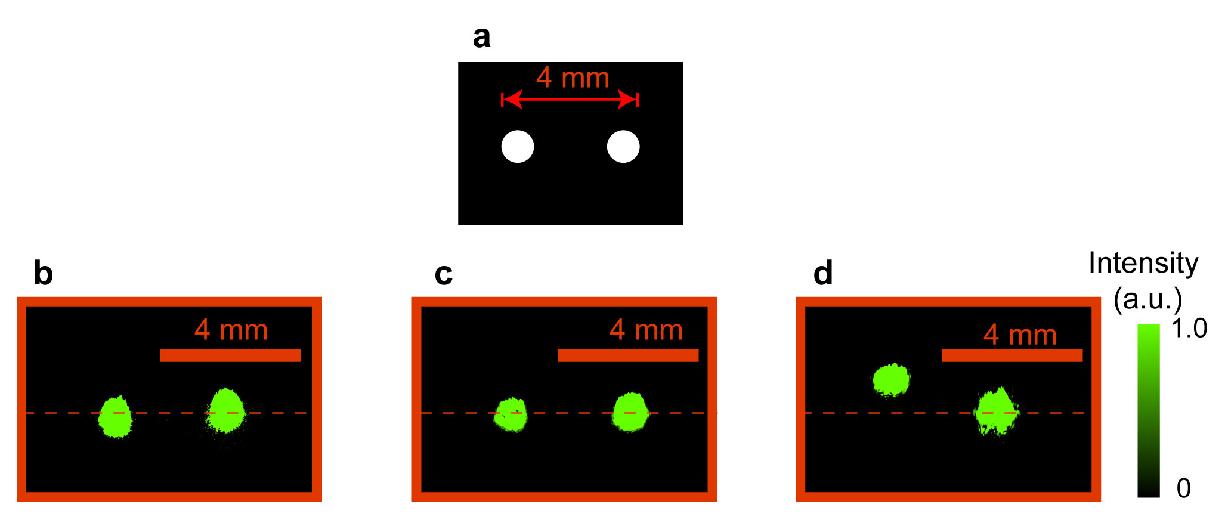
\includegraphics[width=0.8\columnwidth,draft=false]{Fig_5}
\caption{\label{fig:twopoints} Изображения (a) двух пятен, с углами 
падения внутри емкости 
(b) $\theta=0^\circ$, (c) $\theta=18^\circ$ и (d) $\theta=40^\circ$.}
\end{centering}
\end{figure}

После того, как эффективность оболочки был протестирована в условиях зеленого
света (561 нм), цвет был изменен на зеленый (488 нм) и красный (650 нм), 
соответственно. Итоговое изображение на Рис.~\ref{fig:bluered} показывает, что
производительность оболочки все еще остается приемлимо хорошей. Из-за аберрации
цвета, присутствовал сдвиг на 450 микрометров при синем и 400 микрометров при
красном цвете, соответственно, в изображении "M"\ . Сдвиг был меньше, чем 
10\% высоты "M"\ (4.5 мм). Дальнейшая редукция аберрации цвета может быть
достигнута используя методы, вдохновленные комплиментарной 
дисперсией~\cite{lensabberation},
что выходит за пределы рассмотрения этой работы.

Чтобы численно удостовериться в том, что функции нашей оболочки не зависят от
угла падения, мы использовали простой шаблон их двух пятен 
[Рис.~\ref{fig:twopoints}(a)], вместо шаблона "MIT"\ . Длина подсвечивающей
волны снова была рана 561 нм в этом случае. Производительность была проверена
для $\theta = 0^\circ$ и $\theta = 18^\circ$ [Рис.~\ref{fig:twopoints}(b) 
и ~\ref{fig:twopoins}(с)], но в некотором роде упала для $\theta = 40^\circ$
[Рис.~\ref{fig:twopoints}(d)], потому что на таком большом отраженном угле
ошибка в размерностях оболочки увеличивалась. Стоит отметить, что при угле
падения $0^\circ$, свет в действительности не затрагивал низ оболочки или
поверхность стекла. Это соответствует тестированию полного "видения через"\ .

Основное ограничение нашей оболочки на данный момент заключается в том, что
она может работать только в двумерной геометрии (свет должен распространяться
в плоскости, определенной на Рис.~\ref{fig:rays}) и только для одной 
поляризации. Однако, возможно расширить эту оболочку до трехмерной геометрии
точно так же, как двумерную ковровую 
оболочку~\cite{li_carpet,valentine,gabrielli,park} можно расширить до
трехмерной ковровой оболочки~\cite{ergin,huifeng}. 
Так как хорошо известно, что свет,
распространяющийся под водой в основном поляризован с магнитным полем,
параллельным земле, наш дизайн может быть использован в сходных волных средах.
Применение дизайна трансформационной оптики в традиционном построении 
оптических линз является экономически эффективным, но точным решениям для
изготовления скрывающих оболочек. Мы верим, что данная техника откроет 
возможности переведения большего числа устройств, основанных на 
трансформационной оптике, из концепции в плоскость практических применений.

\begin{thebibliography}{22}

\expandafter\ifx\csname
natexlab\endcsname\relax\def\natexlab#1{#1}\fi
\expandafter\ifx\csname bibnamefont\endcsname\relax
  \def\bibnamefont#1{#1}\fi
\expandafter\ifx\csname bibfnamefont\endcsname\relax
  \def\bibfnamefont#1{#1}\fi
\expandafter\ifx\csname citenamefont\endcsname\relax
  \def\citenamefont#1{#1}\fi
\expandafter\ifx\csname url\endcsname\relax
  \def\url#1{\texttt{#1}}\fi
\expandafter\ifx\csname urlprefix\endcsname\relax\def\urlprefix{URL
}\fi \providecommand{\bibinfo}[2]{#2}
\providecommand{\eprint}[2][]{\url{#2}}

\bibitem[1]{huanyang_review}
\bibinfo{author}{\bibfnamefont{H.}~\bibnamefont{Chen}},
  \bibinfo{author}{\bibfnamefont{C.~T.} \bibnamefont{Chan}}, \bibnamefont{and}
  \bibinfo{author}{\bibfnamefont{P.}~\bibnamefont{Sheng}},
  \bibinfo{journal}{Nature Mater.} \textbf{\bibinfo{volume}{9}},
  \bibinfo{pages}{387} (\bibinfo{year}{2010}).

\bibitem[2]{leonhardt}
\bibinfo{author}{\bibfnamefont{U.}~\bibnamefont{Leonhardt}},
  \bibinfo{journal}{Science} \textbf{\bibinfo{volume}{312}},
  \bibinfo{pages}{1777} (\bibinfo{year}{2006}).

\bibitem[3]{pendry}
\bibinfo{author}{\bibfnamefont{J.~B.} \bibnamefont{Pendry}},
  \bibinfo{author}{\bibfnamefont{D.}~\bibnamefont{Schurig}}, \bibnamefont{and}
  \bibinfo{author}{\bibfnamefont{D.~R.} \bibnamefont{Smith}},
  \bibinfo{journal}{Science} \textbf{\bibinfo{volume}{312}},
  \bibinfo{pages}{1780} (\bibinfo{year}{2006}).

\bibitem[4]{leonhardt_broad}
\bibinfo{author}{\bibfnamefont{U.}~\bibnamefont{Leonhardt}} \bibnamefont{and}
  \bibinfo{author}{\bibfnamefont{T.}~\bibnamefont{Tyc}},
  \bibinfo{journal}{Science} \textbf{\bibinfo{volume}{323}},
  \bibinfo{pages}{110} (\bibinfo{year}{2009}).

\bibitem[5]{li_carpet}
\bibinfo{author}{\bibfnamefont{J.}~\bibnamefont{Li}} \bibnamefont{and}
  \bibinfo{author}{\bibfnamefont{J.~B.} \bibnamefont{Pendry}},
  \bibinfo{journal}{Phys. Rev. Lett.} \textbf{\bibinfo{volume}{101}},
  \bibinfo{pages}{203901} (\bibinfo{year}{2008}).

\bibitem[6]{schurig}
\bibinfo{author}{\bibfnamefont{D.}~\bibnamefont{Schurig}},
  \bibinfo{author}{\bibfnamefont{J.~J.} \bibnamefont{Mock}},
  \bibinfo{author}{\bibfnamefont{B.~J.} \bibnamefont{Justice}},
  \bibinfo{author}{\bibfnamefont{S.~A.} \bibnamefont{Cummer}},
  \bibinfo{author}{\bibfnamefont{J.~B.} \bibnamefont{Pendry}},
  \bibinfo{author}{\bibfnamefont{A.~F.} \bibnamefont{Starr}}, \bibnamefont{and}
  \bibinfo{author}{\bibfnamefont{D.~R.} \bibnamefont{Smith}},
  \bibinfo{journal}{Science} \textbf{\bibinfo{volume}{314}},
  \bibinfo{pages}{977} (\bibinfo{year}{2006}).

\bibitem[7]{smolyaninov_SPP}
\bibinfo{author}{\bibfnamefont{I.~I.} \bibnamefont{Smolyaninov}},
  \bibinfo{author}{\bibfnamefont{Y.~J.}~\bibnamefont{Hung}}, \bibnamefont{and}
  \bibinfo{author}{\bibfnamefont{C.~C.} \bibnamefont{Davis}},
  \bibinfo{journal}{Opt. Lett.} \textbf{\bibinfo{volume}{33}},
  \bibinfo{pages}{1342} (\bibinfo{year}{2008}).

\bibitem[8]{ruopeng}
\bibinfo{author}{\bibfnamefont{R.}~\bibnamefont{Liu}},
  \bibinfo{author}{\bibfnamefont{C.}~\bibnamefont{Ji}},
  \bibinfo{author}{\bibfnamefont{J.~J.} \bibnamefont{Mock}},
  \bibinfo{author}{\bibfnamefont{J.~Y.} \bibnamefont{Chin}},
  \bibinfo{author}{\bibfnamefont{T.~J.} \bibnamefont{Cui}}, \bibnamefont{and}
  \bibinfo{author}{\bibfnamefont{D.~R.} \bibnamefont{Smith}},
  \bibinfo{journal}{Science} \textbf{\bibinfo{volume}{323}},
  \bibinfo{pages}{366} (\bibinfo{year}{2009}).

\bibitem[9]{valentine}
\bibinfo{author}{\bibfnamefont{J.}~\bibnamefont{Valentine}},
  \bibinfo{author}{\bibfnamefont{J.}~\bibnamefont{Li}},
  \bibinfo{author}{\bibfnamefont{T.}~\bibnamefont{Zentgraf}},
  \bibinfo{author}{\bibfnamefont{G.}~\bibnamefont{Bartal}}, \bibnamefont{and}
  \bibinfo{author}{\bibfnamefont{X.}~\bibnamefont{Zhang}},
  \bibinfo{journal}{Nature Mater.} \textbf{\bibinfo{volume}{8}},
  \bibinfo{pages}{568} (\bibinfo{year}{2009}).

\bibitem[10]{gabrielli}
\bibinfo{author}{\bibfnamefont{L.~H.} \bibnamefont{Gabrielli}},
  \bibinfo{author}{\bibfnamefont{J.}~\bibnamefont{Cardenas}},
  \bibinfo{author}{\bibfnamefont{C.~B.} \bibnamefont{Poitras}},
  \bibnamefont{and} \bibinfo{author}{\bibfnamefont{M.}~\bibnamefont{Lipson}},
  \bibinfo{journal}{Nature Photon.} \textbf{\bibinfo{volume}{3}},
  \bibinfo{pages}{461} (\bibinfo{year}{2009}).

\bibitem[11]{park}
\bibinfo{author}{\bibfnamefont{J.~H.} \bibnamefont{Lee}},
  \bibinfo{author}{\bibfnamefont{J.}~\bibnamefont{Blair}},
  \bibinfo{author}{\bibfnamefont{V.~A.} \bibnamefont{Tamma}},
  \bibinfo{author}{\bibfnamefont{Q.}~\bibnamefont{Wu}},
  \bibinfo{author}{\bibfnamefont{S.~J.} \bibnamefont{Rhee}},
  \bibinfo{author}{\bibfnamefont{C.~J.} \bibnamefont{Summers}},
  \bibnamefont{and} \bibinfo{author}{\bibfnamefont{W.}~\bibnamefont{Park}},
  \bibinfo{journal}{Opt. Express} \textbf{\bibinfo{volume}{17}},
  \bibinfo{pages}{12922} (\bibinfo{year}{2009}).

\bibitem[12]{smolyaninov_waveguide}
\bibinfo{author}{\bibfnamefont{I.~I.} \bibnamefont{Smolyaninov}},
  \bibinfo{author}{\bibfnamefont{V.~N.} \bibnamefont{Smolyaninova}},
  \bibinfo{author}{\bibfnamefont{A.~V.} \bibnamefont{Kildishev}},
  \bibnamefont{and} \bibinfo{author}{\bibfnamefont{V.~M.}
  \bibnamefont{Shalaev}}, \bibinfo{journal}{Phys. Rev. Lett.}
  \textbf{\bibinfo{volume}{102}}, \bibinfo{pages}{213901}
  (\bibinfo{year}{2009}).

\bibitem[13]{ergin}
\bibinfo{author}{\bibfnamefont{T.}~\bibnamefont{Ergin}},
  \bibinfo{author}{\bibfnamefont{N.}~\bibnamefont{Stenger}},
  \bibinfo{author}{\bibfnamefont{P.}~\bibnamefont{Brenner}},
  \bibinfo{author}{\bibfnamefont{J.~B.} \bibnamefont{Pendry}},
  \bibnamefont{and} \bibinfo{author}{\bibfnamefont{M.}~\bibnamefont{Wegener}},
  \bibinfo{journal}{Science} \textbf{\bibinfo{volume}{328}},
  \bibinfo{pages}{337} (\bibinfo{year}{2010}).

\bibitem[14]{huifeng}
\bibinfo{author}{\bibfnamefont{H.~F.} \bibnamefont{Ma}} \bibnamefont{and}
  \bibinfo{author}{\bibfnamefont{T.~J.} \bibnamefont{Cui}},
  \bibinfo{journal}{Nat. Commun.} p. \bibinfo{pages}{1:21
  doi:10.1038/ncomms1023} (\bibinfo{year}{2010}).

\bibitem[15]{baile_rainbow}
\bibinfo{author}{\bibfnamefont{B.}~\bibnamefont{Zhang}},
  \bibinfo{author}{\bibfnamefont{B.-I.} \bibnamefont{Wu}},
  \bibinfo{author}{\bibfnamefont{H.}~\bibnamefont{Chen}}, \bibnamefont{and}
  \bibinfo{author}{\bibfnamefont{J.~A.} \bibnamefont{Kong}},
  \bibinfo{journal}{Phys. Rev. Lett.} \textbf{\bibinfo{volume}{101}},
  \bibinfo{pages}{063902} (\bibinfo{year}{2008}).

\bibitem[16]{baile_lateral_shift}
\bibinfo{author}{\bibfnamefont{B.}~\bibnamefont{Zhang}},
  \bibinfo{author}{\bibfnamefont{T.}~\bibnamefont{Chan}}, \bibnamefont{and}
  \bibinfo{author}{\bibfnamefont{B.-I.} \bibnamefont{Wu}},
  \bibinfo{journal}{Phys. Rev. Lett.} \textbf{\bibinfo{volume}{104}},
  \bibinfo{pages}{233903} (\bibinfo{year}{2010}).

\bibitem[17]{xisheng}
\bibinfo{author}{\bibfnamefont{S.}~\bibnamefont{Xi}},
  \bibinfo{author}{\bibfnamefont{H.}~\bibnamefont{Chen}},
  \bibinfo{author}{\bibfnamefont{B.-I.} \bibnamefont{Wu}}, \bibnamefont{and}
  \bibinfo{author}{\bibfnamefont{J.~A.} \bibnamefont{Kong}},
  \bibinfo{journal}{IEEE Microw. Wireless Compon. Lett.}
  \textbf{\bibinfo{volume}{19}}, \bibinfo{pages}{131} (\bibinfo{year}{2009}).

\bibitem[18]{zhang10}
\bibinfo{author}{\bibfnamefont{B.}~\bibnamefont{Zhang}},
  \bibinfo{author}{\bibfnamefont{Y.}~\bibnamefont{Luo}},
  \bibinfo{author}{\bibfnamefont{X.} \bibnamefont{Liu}}, \bibnamefont{and}
  \bibinfo{author}{\bibfnamefont{G.} \bibnamefont{Barbastathis}},
  \bibinfo{journal}{arXiv.org}
  \textbf{\bibinfo{volume}{1012}}, \bibinfo{pages}{2238} (\bibinfo{year}{2010}).

\bibitem[19]{chen10}
\bibinfo{author}{\bibfnamefont{X.}~\bibnamefont{Chen}},
  \bibinfo{author}{\bibfnamefont{Y.}~\bibnamefont{Luo}},
  \bibinfo{author}{\bibfnamefont{J.} \bibnamefont{Zhang}},
  \bibinfo{author}{\bibfnamefont{K.} \bibnamefont{Jiang}},
  \bibinfo{author}{\bibfnamefont{J.~B.} \bibnamefont{Pendry}},
  \bibnamefont{and}
  \bibinfo{author}{\bibfnamefont{S.} \bibnamefont{Zhang}},
  \bibinfo{journal}{arXiv.org}
  \textbf{\bibinfo{volume}{1012}}, \bibinfo{pages}{2783} (\bibinfo{year}{2010}).

\bibitem[20]{wyszecki}
\bibinfo{author}{\bibfnamefont{G.}~\bibnamefont{Wyszecki}} \bibnamefont{and}
  \bibinfo{author}{\bibfnamefont{W.~S.} \bibnamefont{Stiles}},
  \emph{\bibinfo{title}{Color Science: Concepts and Methods, Quantitative Data
  and Formulas,}} (\bibinfo{publisher}{Wiley, New York}, \bibinfo{year}{2000}).

\bibitem[21]{hashemi}
\bibinfo{author}{\bibfnamefont{H.}~\bibnamefont{Hashemi}},
  \bibinfo{author}{\bibfnamefont{B.}~\bibnamefont{Zhang}},
  \bibinfo{author}{\bibfnamefont{J.~D.} \bibnamefont{Joannopoulos}},
  \bibnamefont{and} \bibinfo{author}{\bibfnamefont{S.~G.}
  \bibnamefont{Johnson}}, \bibinfo{journal}{Phys. Rev. Lett.}
  \textbf{\bibinfo{volume}{104}}, \bibinfo{pages}{253903}
  (\bibinfo{year}{2010}).

\bibitem[22]{lensabberation}
\bibinfo{author}{\bibfnamefont{H.}~\bibnamefont{Gross}},
  \bibinfo{author}{\bibfnamefont{H.}~\bibnamefont{Zugge}},
  \bibinfo{author}{\bibfnamefont{M.}~\bibnamefont{Peschka}}, \bibnamefont{and}
  \bibinfo{author}{\bibfnamefont{F.}~\bibnamefont{Blechinger}},
  \emph{\bibinfo{title}{Handboook of Optical Systems, Volume 3: Aberration
  Theory and Correction of Optical Systems,}} (\bibinfo{publisher}{Wiley-VCH,
  Weinheim}, \bibinfo{year}{2007}).

\end{thebibliography}
\end{document}